\documentclass[12pt,a4paper]{article}
\usepackage[margin=1in]{geometry}
\usepackage{amsmath}
\usepackage{listings}
\usepackage{xcolor}
\usepackage{graphicx}

\begin{document}

\pagenumbering{gobble}

\section*{Hill Cipher: Theoretical Overview}

\subsection*{Hill Cipher}

The Hill cipher is a polygraphic substitution cipher based on linear algebra, invented by Lester S. Hill in 1929. It was the first polygraphic cipher in which it was practical to operate on more than three symbols at once.

\subsubsection*{Encryption}

To encrypt a message, each block of $n$ letters (considered as an $n$-component vector) is multiplied by an invertible $n \times n$ matrix, against a modulus that depends on the size of the alphabet (26 for the English alphabet). Each letter is represented by a number modulo 26, with A=0, B=1, \ldots, Z=25.

For example, consider the message 'ACT' and the key matrix:
\[
\begin{pmatrix}
6 & 24 & 1 \\
13 & 16 & 10 \\
20 & 17 & 15
\end{pmatrix}
\]

Since 'A' is 0, 'C' is 2, and 'T' is 19, the message can be written as the vector:
\[
\begin{pmatrix}
0 \\
2 \\
19
\end{pmatrix}
\]

The enciphered vector is then obtained by matrix multiplication:
\[
\begin{pmatrix}
6 & 24 & 1 \\
13 & 16 & 10 \\
20 & 17 & 15
\end{pmatrix}
\begin{pmatrix}
0 \\
2 \\
19
\end{pmatrix}
=
\begin{pmatrix}
67 \\
222 \\
319
\end{pmatrix}
\equiv 
\begin{pmatrix}
15 \\
14 \\
7
\end{pmatrix} \pmod {26}
\]

which corresponds to a ciphertext of 'POH'.

\subsubsection*{Decryption}

To decrypt a message, we turn the ciphertext back into a vector and multiply it by the inverse of the key matrix used for encryption.

For example, using the same key matrix as above, the inverse matrix is:
\[
\begin{pmatrix}
6 & 24 & 1 \\
13 & 16 & 10 \\
20 & 17 & 15
\end{pmatrix}^{-1}
\equiv 
\begin{pmatrix}
8 & 5 & 10 \\
21 & 8 & 21 \\
21 & 12 & 8
\end{pmatrix} \pmod {26}
\]

If we have the ciphertext 'POH', we can decrypt it as follows:
\[
\begin{pmatrix}
8 & 5 & 10 \\
21 & 8 & 21 \\
21 & 12 & 8
\end{pmatrix}
\begin{pmatrix}
15 \\
14 \\
7
\end{pmatrix}
=
\begin{pmatrix}
260 \\
574 \\
539
\end{pmatrix}
\equiv 
\begin{pmatrix}
0 \\
2 \\
19
\end{pmatrix} \pmod {26}
\]

which gets us back to 'ACT'.

\subsubsection*{Choosing the Key Matrix}

Not all matrices can be used as key matrices in the Hill cipher. The determinant of the matrix must be non-zero and must not have any common factors with the modular base (26 for the English alphabet). This ensures that the matrix is invertible, which is necessary for decryption.

For example, the determinant of the 3x3 key matrix above is:
\[
\begin{vmatrix}
6 & 24 & 1 \\
13 & 16 & 10 \\
20 & 17 & 15
\end{vmatrix}
= 6(16 \cdot 15 - 10 \cdot 17) - 24(13 \cdot 15 - 10 \cdot 20) + 1(13 \cdot 17 - 16 \cdot 20) = 441 \equiv 25 \pmod {26}
\]

Since 25 is prime with 26 (i.e., they have no common factors), this matrix can be used for the Hill cipher.

\subsubsection*{Variants and Extensions}

The basic Hill cipher is vulnerable to known-plaintext attacks because it is completely linear. However, it can be combined with other non-linear operations to increase its security. For example, the MixColumns step in AES is a matrix multiplication, and the Twofish cipher uses a combination of non-linear S-boxes with a carefully chosen matrix multiplication.

The Hill cipher can also be extended to work with larger blocks of letters by using larger key matrices. Hill himself invented a machine that mechanically implemented a 6 x 6 version of the cipher, which was very secure. However, the machine was unable to change the key setting, limiting its use in practice.

\newpage

\lstinputlisting[caption=hill-cipher.py,language=Python,basicstyle=\ttfamily\footnotesize, captionpos=t, numbers=left, breaklines=true]{hill-cipher.py}

\newpage

\begin{figure}[h]
    \caption{Output}
    \centering
    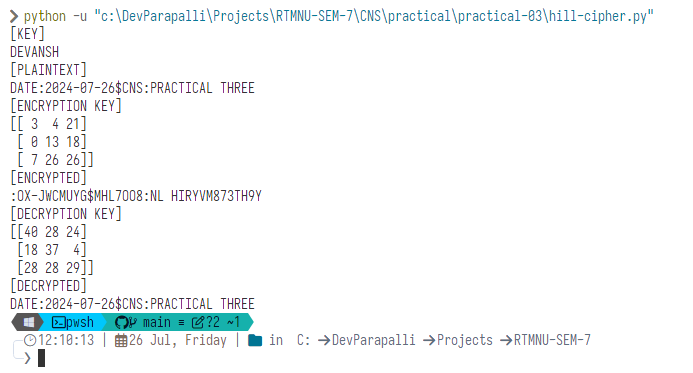
\includegraphics[width=\textwidth]{output.png}
\end{figure}


% \begin{center}
%     \textbf{Output}
%     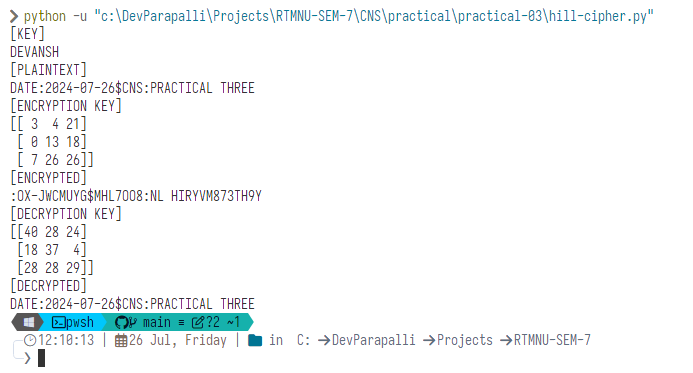
\includegraphics[width=\textwidth]{output.png}
% \end{center}

\end{document}